\chapter{The LSND and MiniBooNE anomalies}

\minitoc

This chapter will describe experimental apparatus and the results of the LSND and MiniBooNE experiments. The LSND experiment observed an excess of $\bar{\nu}_{e}$ in a primarily $\bar{\nu}_{\mu}$ beam in 2001. The MiniBooNE experiment, built to confirm or rule out the anomaly, observed a significant excess of $\nu_{e}$-like ($\bar{\nu}_{e}$-like) events in a primarily $\nu_{\mu}$ ($\bar{\nu}_{\mu}$) beam. A discussion of the possible physics explanation for the excess will also be provided.

\section{The LSND experiment}
The Liquid Scintillator Neutrino Detector (LSND) was an experiment at the Los Alamos National Laboratory which aimed to detect $\bar{\nu}_e$ interactions in a mainly $\bar{\nu}_{\mu}$ beam. The neutrino beam was produced by firing a 800 MeV proton beam into a target, producing charged pions, which were stopped in a beam dump. The $\pi^-$ part was electromagnetically captured by the nucleus, while the $\pi^+$ component initiated the decay chain:
\begin{align}
    \pi^+ \rightarrow & \mu^+\nu_{\mu}\\
    & \rotatebox[origin=c]{180}{$\Lsh$}	 \mu^{+} \rightarrow e^+\bar{\nu}_{\mu}\nu_{e},
\end{align}
which created an almost pure beam of $\bar{\nu}_{\mu}$, $\nu_{\mu}$, and $\nu_e$.

The $\bar{\nu}_e$ interactions were detected via an inverse $\beta$-decay process in the liquid scintillator and tagged with a delayed coincidence between the positron and the subsequent neutron capture, in a fashion similar to the Cowan and Reines experiment. 

LSND found an excess of $\bar{\nu}_e$ interactions with a significance $>3\sigma$, which could be explained as $\bar{\nu}_\mu$ oscillating into $\bar{\nu}_e$ (Figure \ref{fig:resultlsnd}). Given the $L/E\approx0.75$~m/MeV of the experiment, the mass splitting term obtained with LSND data is $\Delta m_{\mathrm{LSND}}^2\approx1$~eV. This value is one order of magnitude larger than the mass splitting terms obtained with any other reactor, accelerator, atmospheric, or solar experiment \cite{Aguilar:2001ty}. 

\begin{figure}[htbp]
  \begin{subfigure}{0.45\textwidth}
    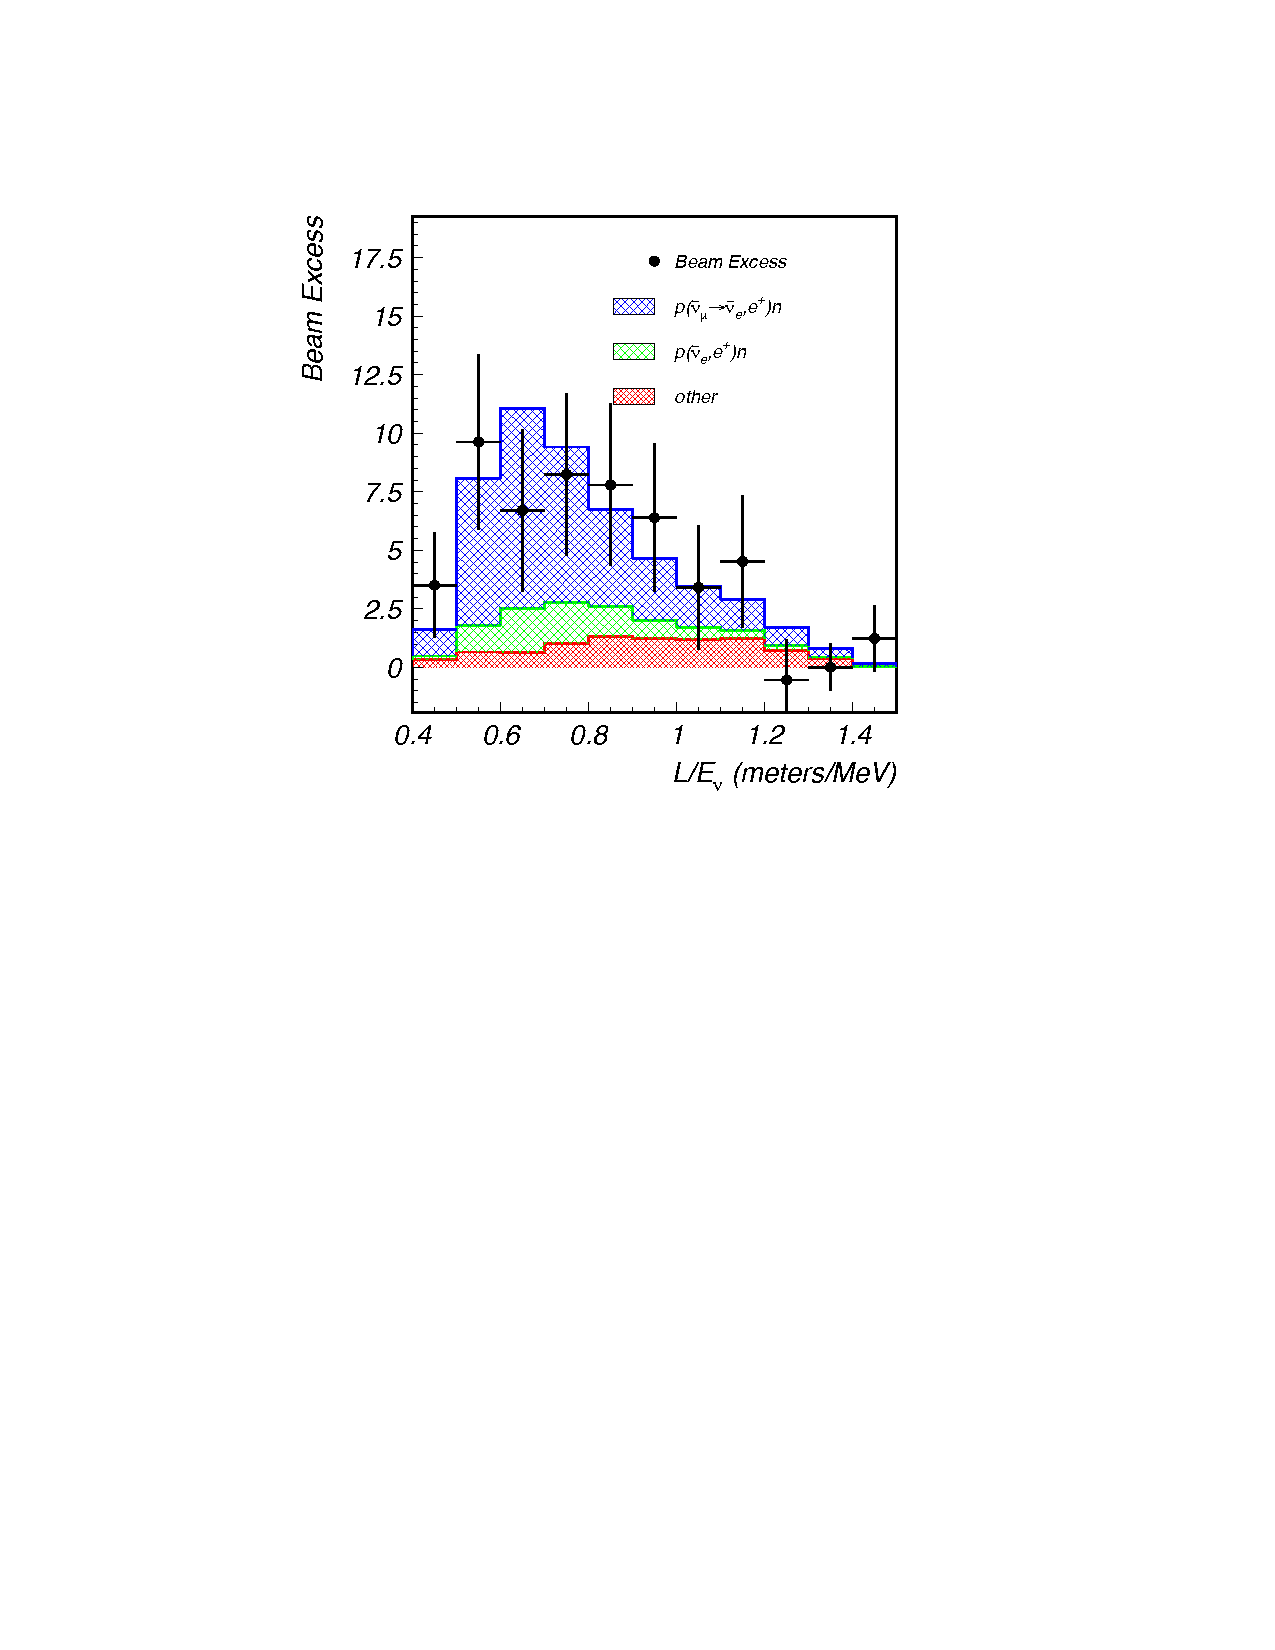
\includegraphics[height=\linewidth]{figures/lsndresult.pdf}
    \caption{$L/E_{\nu}$ distribution for the $\bar{\nu}_{e}$ events in the LSND experiment.}\label{fig:resultlsnd}
  \end{subfigure}\hfill
  \begin{subfigure}{0.45\textwidth}
    \begin{center}
        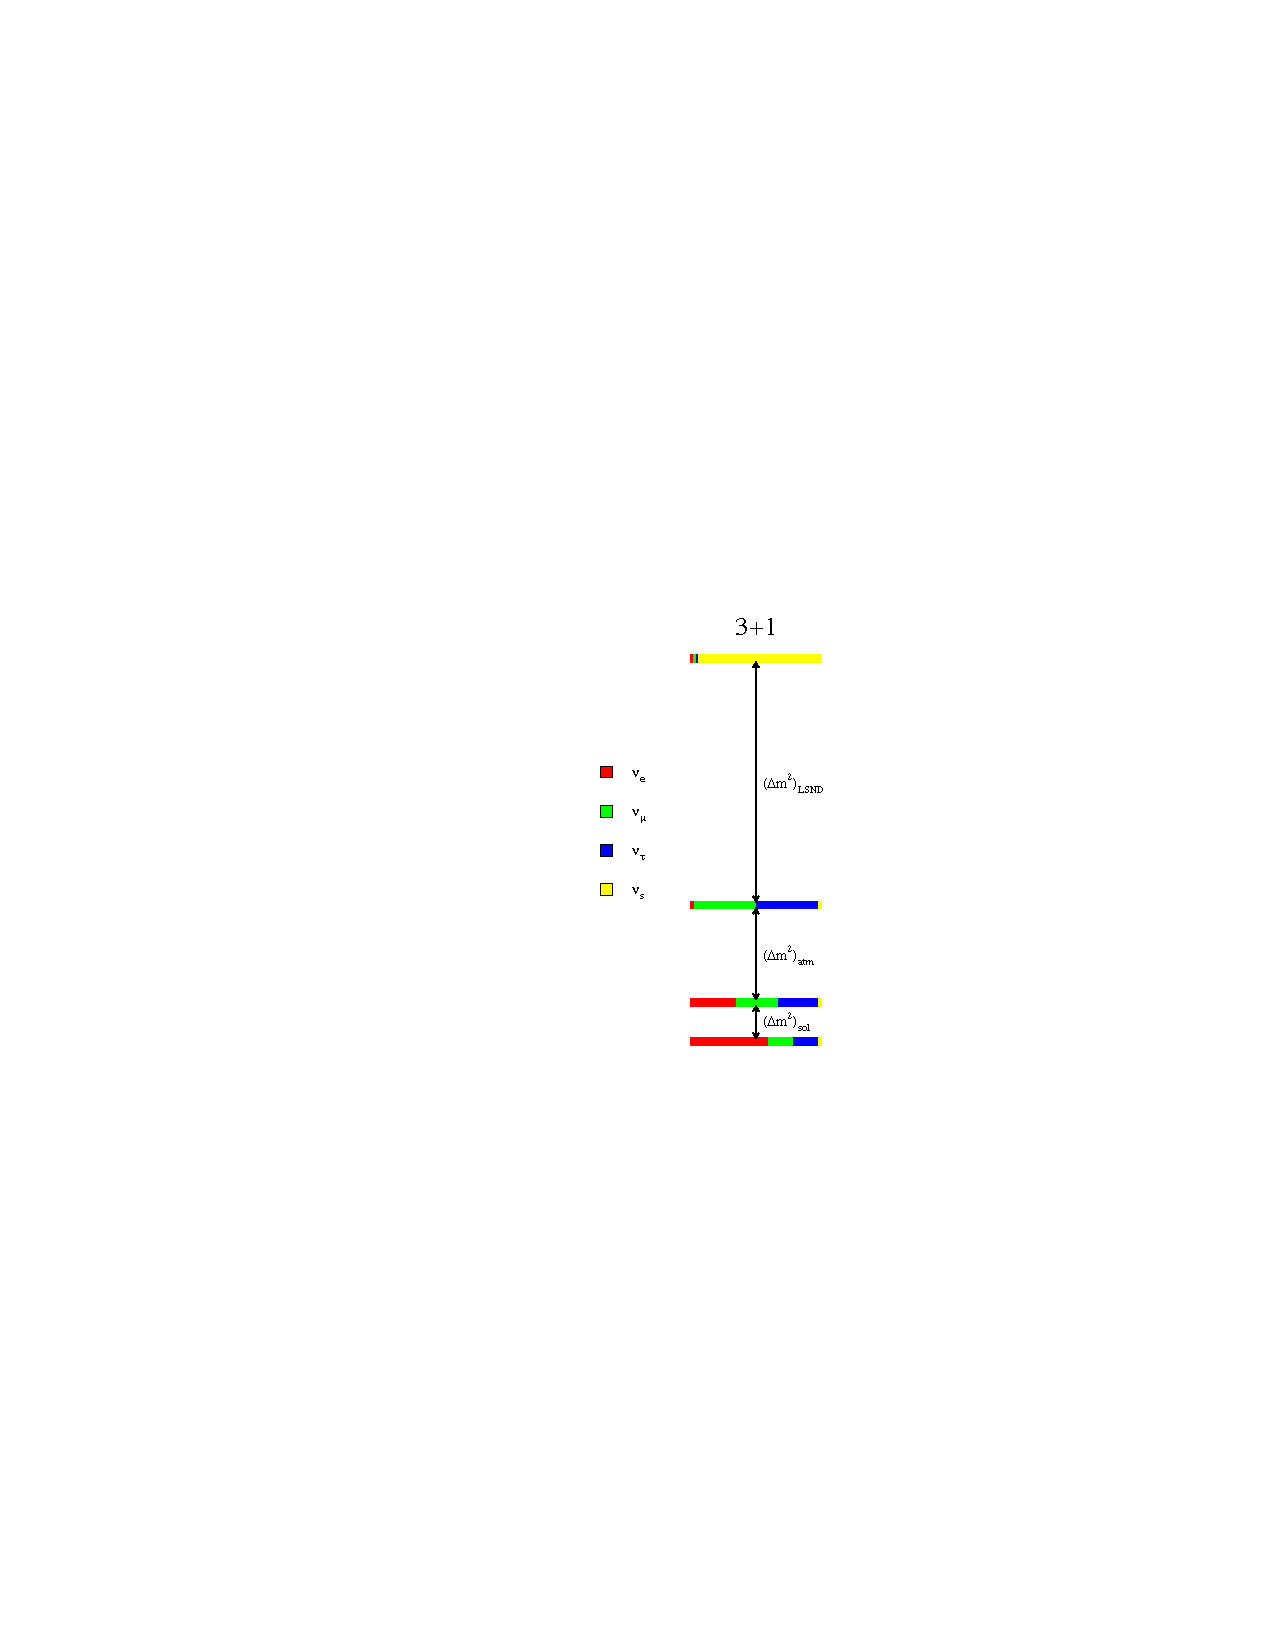
\includegraphics[height=\linewidth]{figures/masslsnd.pdf}
        \caption{Neutrino mass normal hierarchy in the scenario of 3+1 neutrinos.}\label{fig:masslsnd}
    \end{center}
  \end{subfigure}
    \caption{The excess of electron antineutrinos observed by the LSND experiment (left) can be interpreted with the presence of a fourth neutrino state, with a mass splitting term larger than $(\Delta m^2)_{\mathrm{atm}}$ and $(\Delta m^2)_{\mathrm{sol}}$ (right).}
\end{figure}

A proposed solution to the LSND anomaly is to have one additional neutrino state, which would mix with the standard three neutrinos, in a 3+1 scenario. This fourth neutrino is often called \emph{sterile}, because it does not interact with the $Z$ boson (since its width is compatible only with $N_{\nu}=3$. The PMNS matrix in this case will have an extra dimension ($4\times4$) and the sterile mass neutrino eigenstate will be written as:
\begin{equation}
    \ket{\nu_s}=\sum^{3+1}_{\alpha}U_{i,\alpha}\ket{\nu_{\alpha}}.
\end{equation}
A diagram of the mass hierarchy in this scenario is shown in Figure \ref{fig:masslsnd}.

Figure \ref{fig:globalfit} shows the global fit of the mixing angles and mass splitting terms using the data coming from the main neutrino detection experiments. It is possible to identify two mass-splitting terms and three mixing angles, compatible with a scenario of 3 neutrino flavours, while the LSND allowed region is clearly exploring a completely different region of the parameter space. 

Several experiments after LSND explored the same region: in particular, the KARMEN collaboration employed an experimental setup similar to LSND but it found no significant excess and ruled out a large subset of the LSND parameter space \cite{Eitel:2000by}. A proposed solution to the tension between LSND and other neutrino experiments is to introduce more than one sterile neutrinos. A (3+2) model fits better the existing data than the (3+1) scenario \cite{Sorel:2003hf}.

\begin{figure}[htbp]
    \centering
    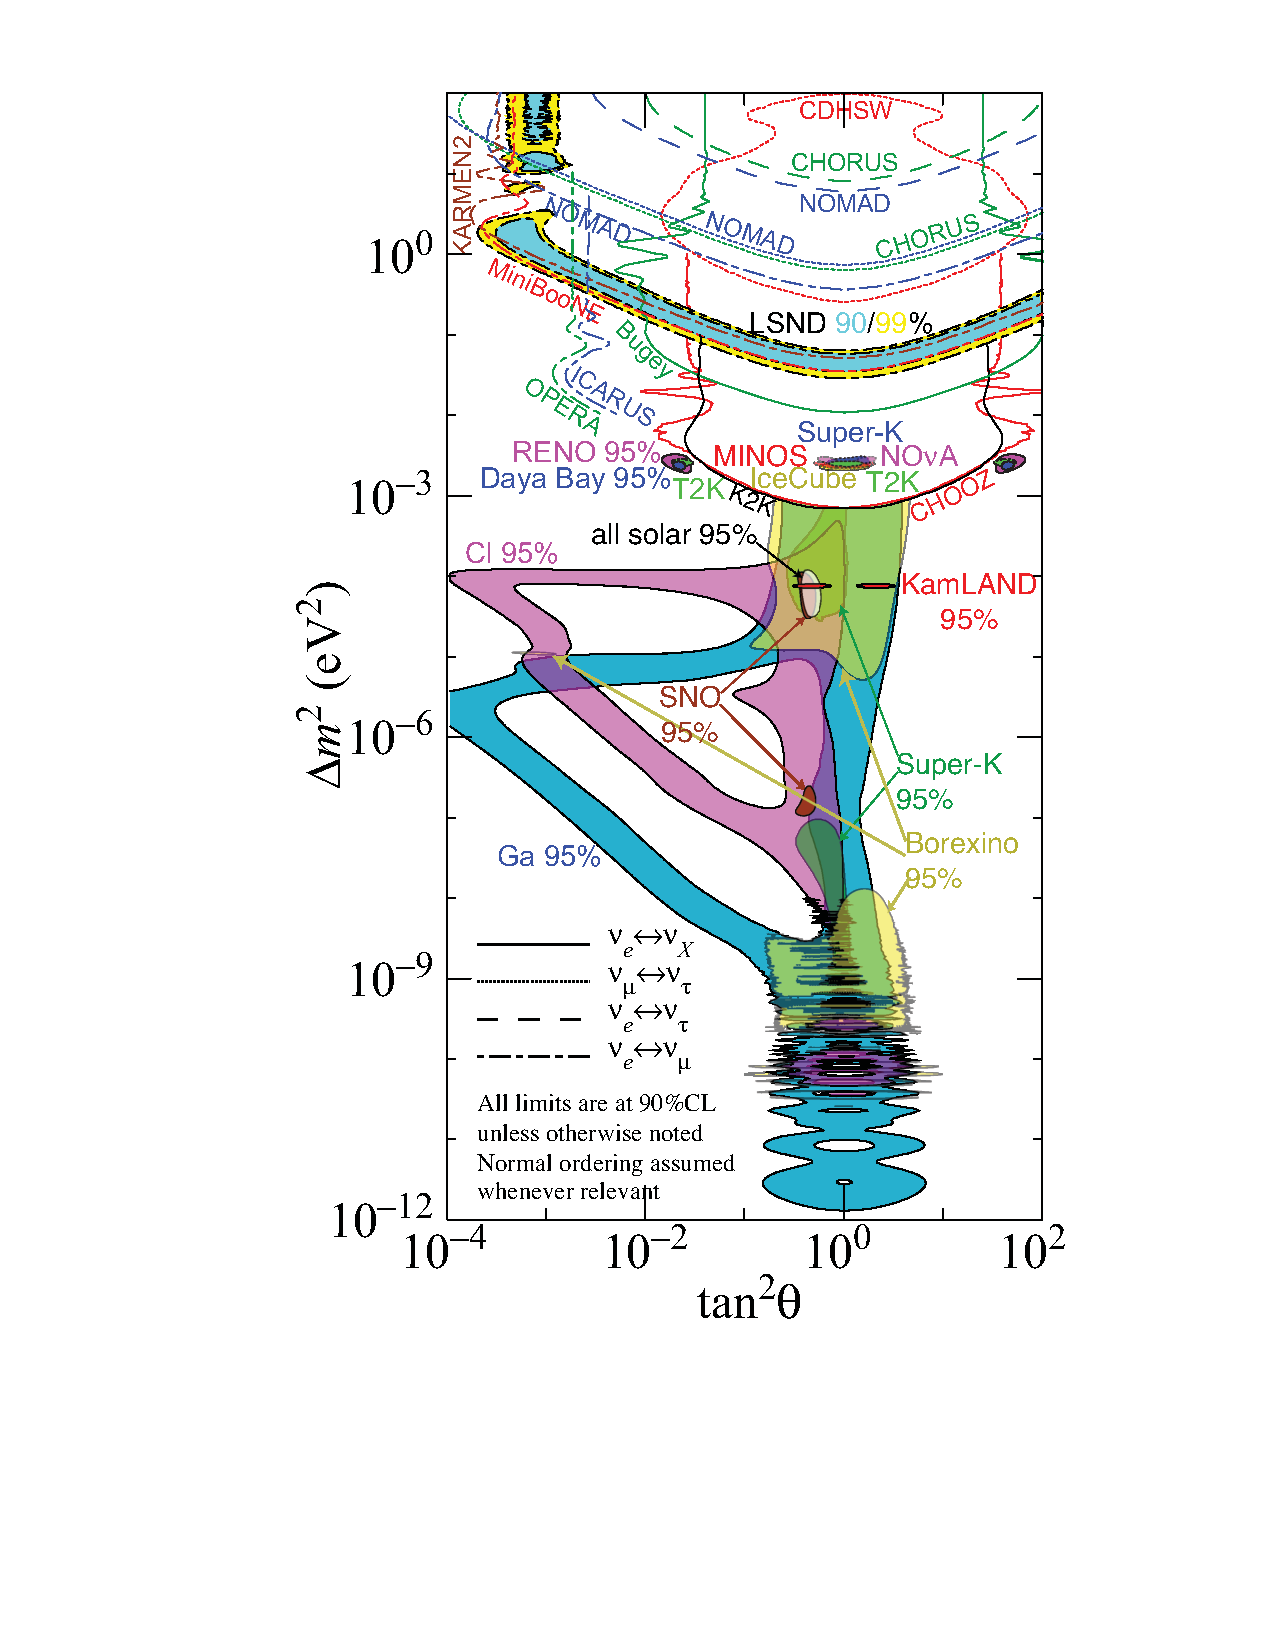
\includegraphics[width=0.7\linewidth]{figures/globalfit.pdf}
    \caption{The squared-mass splittings and mixing angles favoured (solid regions) or excluded (open regions) by existing neutrino oscillation measurements. Results are categorised by channels: $\nu_e$ disappearance (solid lines), $\nu_{\mu} \leftrightarrow \nu_{\tau}$  (dotted lines), $\nu_{e} \leftrightarrow \nu_{\tau}$ (dashed lines), and $\nu_{e} \leftrightarrow \nu_{\mu}$ (dashed-dotted lines). The normal mass ordering is assumed where relevant. Adapted from \cite{PhysRevD.98.030001}. Does not include MiniBooNE latest result \cite{Aguilar-Arevalo:2018gpe}.}
    \label{fig:globalfit}
\end{figure}

\section{The MiniBooNE experiment}
The MiniBooNE experiment was designed to definitely test the LSND result. It consists of a spherical detector filled with mineral oil and located 541 meters downstream of the Booster Neutrino Beam (BNB) production target at Fermilab. This beam can run both in neutrino mode, producing a mainly $\nu_{\mu}$ beam, and in antineutrino mode, producing a mainly $\bar{\nu}_{\mu}$ beam. The BNB neutrino flux is described in detail by the MiniBooNE collaboration in \cite{AguilarArevalo:2008yp}.

The detector is equipped with 1280 8-inch photomultiplier tubes (PMTs) and employs a separated outer veto region with an extra 240 PMTs for cosmic-ray rejection. Particles interacting in the mineral oil produce Cherenkov light, if above detection threshold. The particle identification is based on the different light patterns that each particle produces in the detector: in particular, high-penetrating, heavy particles such as muons will produce sharp rings of Cherenkov light, while lighter particles like electrons and photons will produce fuzzier rings. Neutral pion will instead produce two fuzzy rings partially overlapping when it decays to two photons ($\pi^{0}\rightarrow 2\gamma$). 
This technique introduces an irreducible degeneracy of the particles in the final state, since it is not possible to distinguish a single photon from an electron. 

Energy calibration at MiniBooNE was performed with \emph{in situ} measurement. Cosmic rays, detected with an external hodoscope, and stopping in the mineral oil will produce the typical Michel electron spectrum peaked around $\approx m_{\mu}/2 = 52.8$~MeV. The invariant mass of $\pi^0$ decays can also be reconstructed to measure the energy response around $\approx135$~MeV. 

The oscillation analysis of the MiniBooNE experiment looked for $\nu_e$ charged-current quasi-elastic (CCQE) interactions, where the $\nu_{e}$ exchanges a charged $W$ boson with a neutron in the nucleus, producing an outgoing electron and a proton.
However, hadrons exiting the nucleus after the neutrino interaction can re-interact and change identity or eject other hadrons (Final State Interactions, FSI) \cite{Martini:2013sha}. A neutrino experiment as MiniBooNE, however, cannot observe directly the FSI and, as such, the selected events are called \emph{CCQE-like}, since this definition relies only on the particles in the final state \cite{Katori:2013nca}. 

The energy of the CCQE-like interaction $E_{\nu}^{QE}$ is determined by the electron scattering angle $\theta$ and energy $E_e$, in the approximation of nucleon at rest, as:
\begin{equation}
    E_{\nu}^{QE} = \frac{2m_n E_e + m_p^2- m_n^2 - m_e^2}{2(m_n - E_e + \cos\theta\sqrt{E_e^2-m_e^2})},
\end{equation}
where $m_n$, $m_p$, and $m_e$ are the mass of the neutron, the proton, and the electron, respectively.

\begin{figure}[htbp]
  \begin{subfigure}{0.48\textwidth}
    \begin{center}
    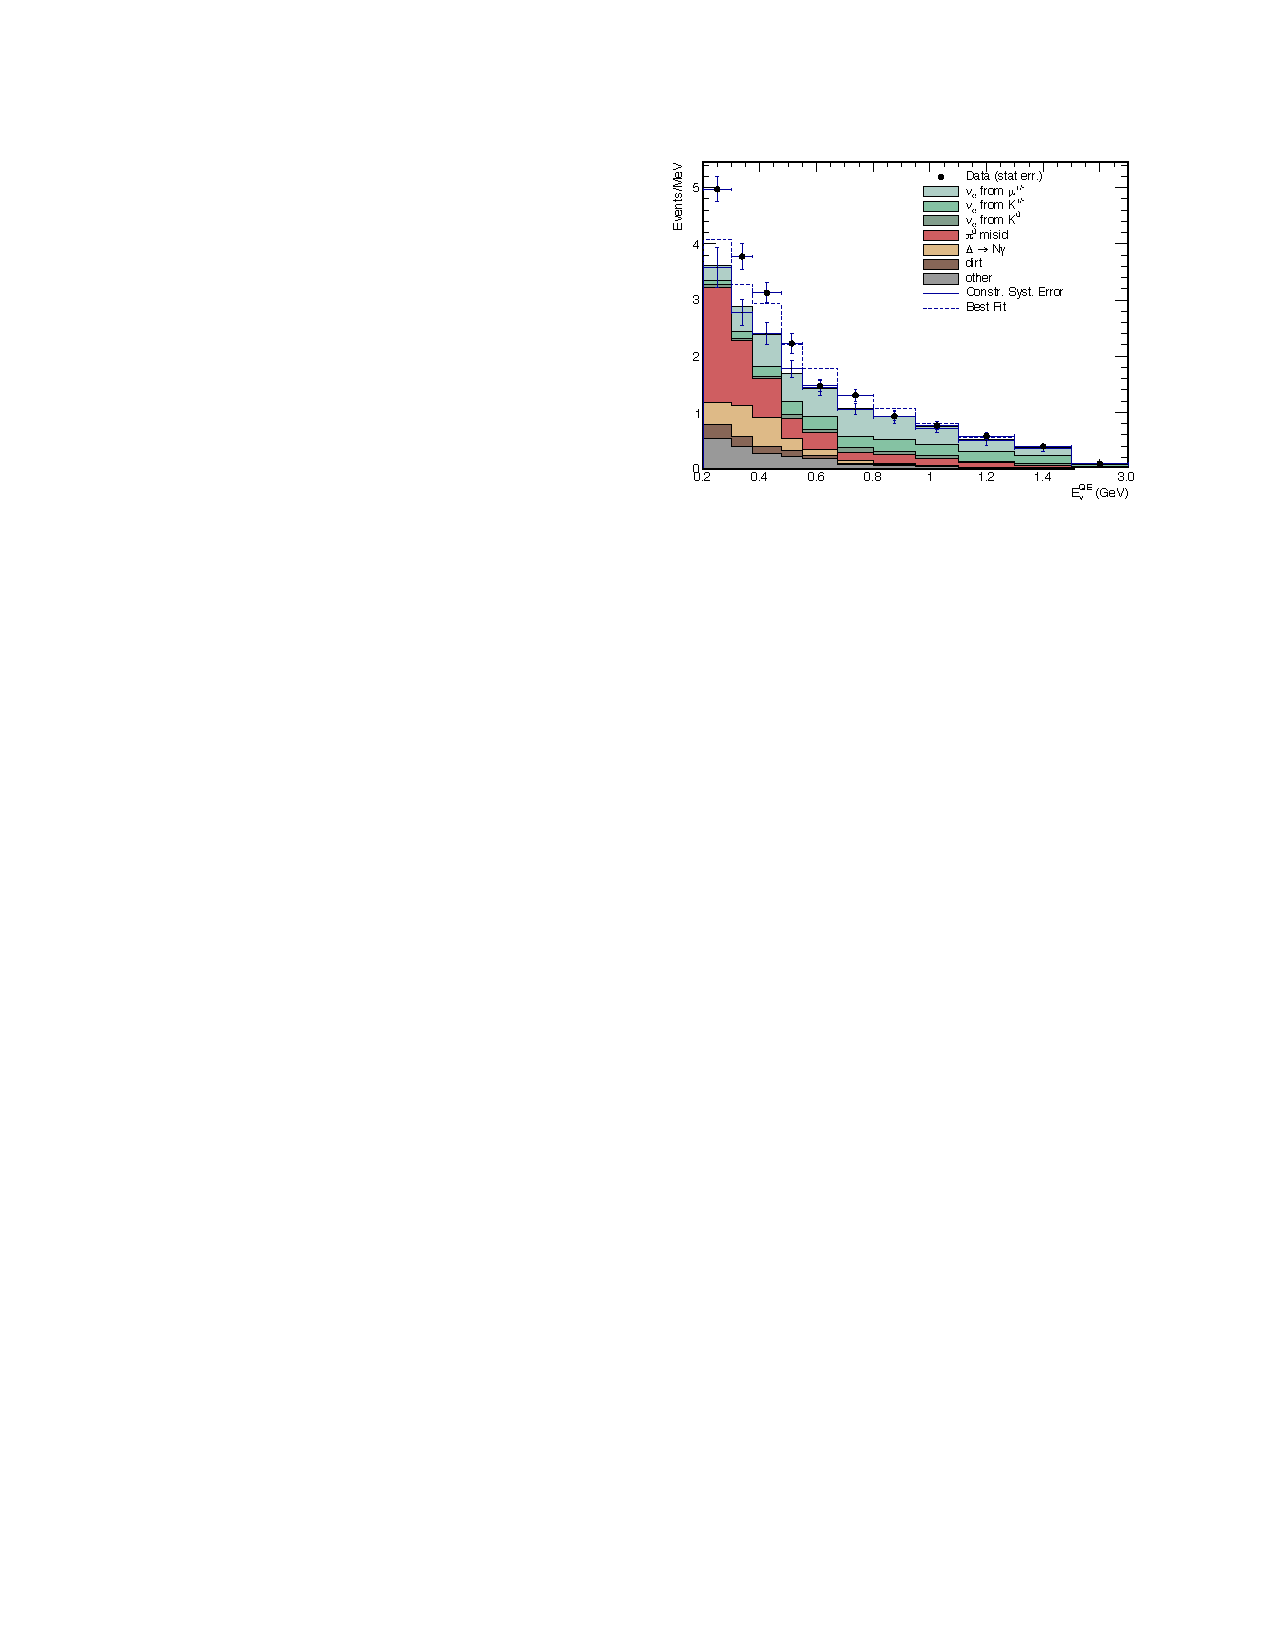
\includegraphics[width=\linewidth]{figures/miniboone_plot.pdf}
    \caption{$E_{\nu}^{QE}$ spectrum in neutrino mode.}
    \label{fig:miniboone_spectrum}
    \end{center}
  \end{subfigure}\hfill
  \begin{subfigure}{0.48\textwidth}
    \begin{center}
    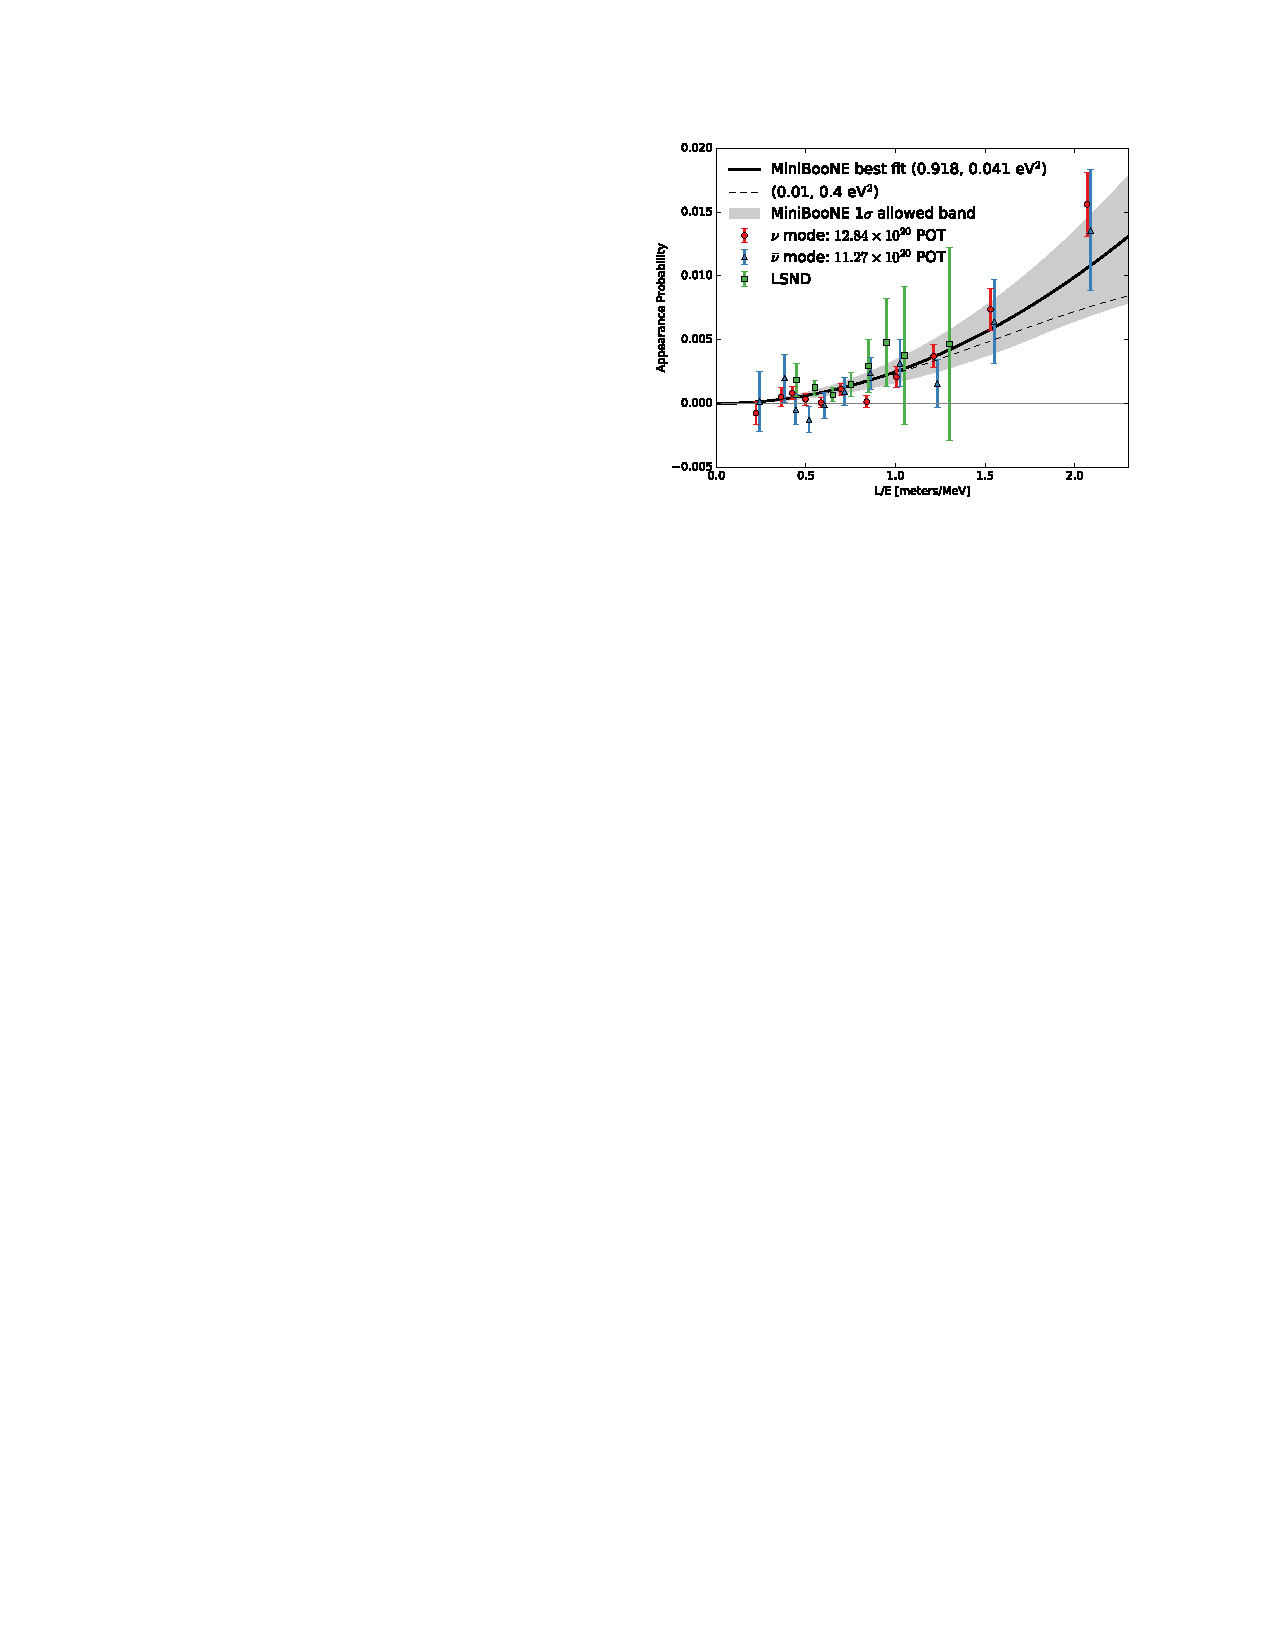
\includegraphics[width=\linewidth]{figures/miniboone_lsnd.pdf}
    \caption{Appearance probability.}
    \label{fig:miniboone_lsnd}
    \end{center}
  \end{subfigure}
  \caption{The MiniBooNE neutrino mode corresponding to the total $12.84\times10^{20}$ POT data, for $\nu_e$ CCQE data (points with statistical errors) and background (histogram with systematic errors). The dashed line represent the two-neutrino model best fit (left). The appearance probability is in agreement with LSND data (right). Adapted from \cite{Aguilar-Arevalo:2018gpe}.}
\end{figure}


The most recent result by the MiniBooNE collaboration \cite{Aguilar-Arevalo:2018gpe} shows a $4.7\sigma$ excess in the combined $\nu_{e}$ and $\bar{\nu}_{e}$ analysis. The energy spectrum of the selected events is shown in Figure \ref{fig:miniboone_spectrum}. The excess of data events is in the sub-GeV energy region and consistent in energy and magnitude with the LSND result. The two excess combined gives a significance of $6.0\sigma$. Figure \ref{fig:miniboone_lsnd} shows the agreement of the appearance probability as a function of the $L/E$ distribution for LSND and MiniBooNE. 

\subsection*{MiniBooNE backgrounds}
The background of the MiniBooNE experiment can be divided into four main categories:
\begin{description}
    \item[Intrinsic $\nu_e$.] The $\nu_e$ component of the beam, coming from $\mu^{\pm}$, $K^{\pm}$, and $K^0$, is the irreducible background of the experiment, since it can't be distinguished from $\nu_{\mu}$ oscillating into $\nu_{e}$. This component of the flux is constrained by measuring the $\nu_{\mu}$ interactions.
    \item[Misidentified $\pi^0$.] The background from misidentified $\pi^0$ events represents the largest component. These events are particularly challenging to reconstruct, since very forward-boosted photons will appear in the detector as a single fuzzy ring. The MiniBooNE collaboration has constrained this contribution by reconstructing the invariant $\pi^0$ mass of the event and obtaining a sample with a purity $>90\%$ of NC $\pi^0$ events. The total uncertainty on the NC background is 7\% \cite{Karagiorgi:2010zz}.
    \item[Misidentified $\Delta\rightarrow N\gamma$.] The production of $\Delta$ resonances is also constrained by the NC $\pi^0$ \emph{in situ} measurement, times the branching fraction of $(0.56\pm0.04)\%$ \cite{PhysRevD.98.030001}. The uncertainty on this component is 12\%.
    \item[Dirt.] The dirt background, meaning neutrino interactions happening outside the detector but where at at least one particle in the final states interacts inside, is also constrained with an \emph{in situ} measurement, where events reconstructed close to the detector boundaries and pointing inwards are selected. 
\end{description}


\subsection*{MiniBooNE result in the two-neutrino oscillation model}

Several new physics scenarios have been hypothesised which could explain the excess. Figure \ref{fig:miniboone_bestfit} shows the MiniBooNE allowed regions in neutrino and antineutrino mode for the two-neutrino oscillation model. 

\begin{figure}[htbp]
    \centering
    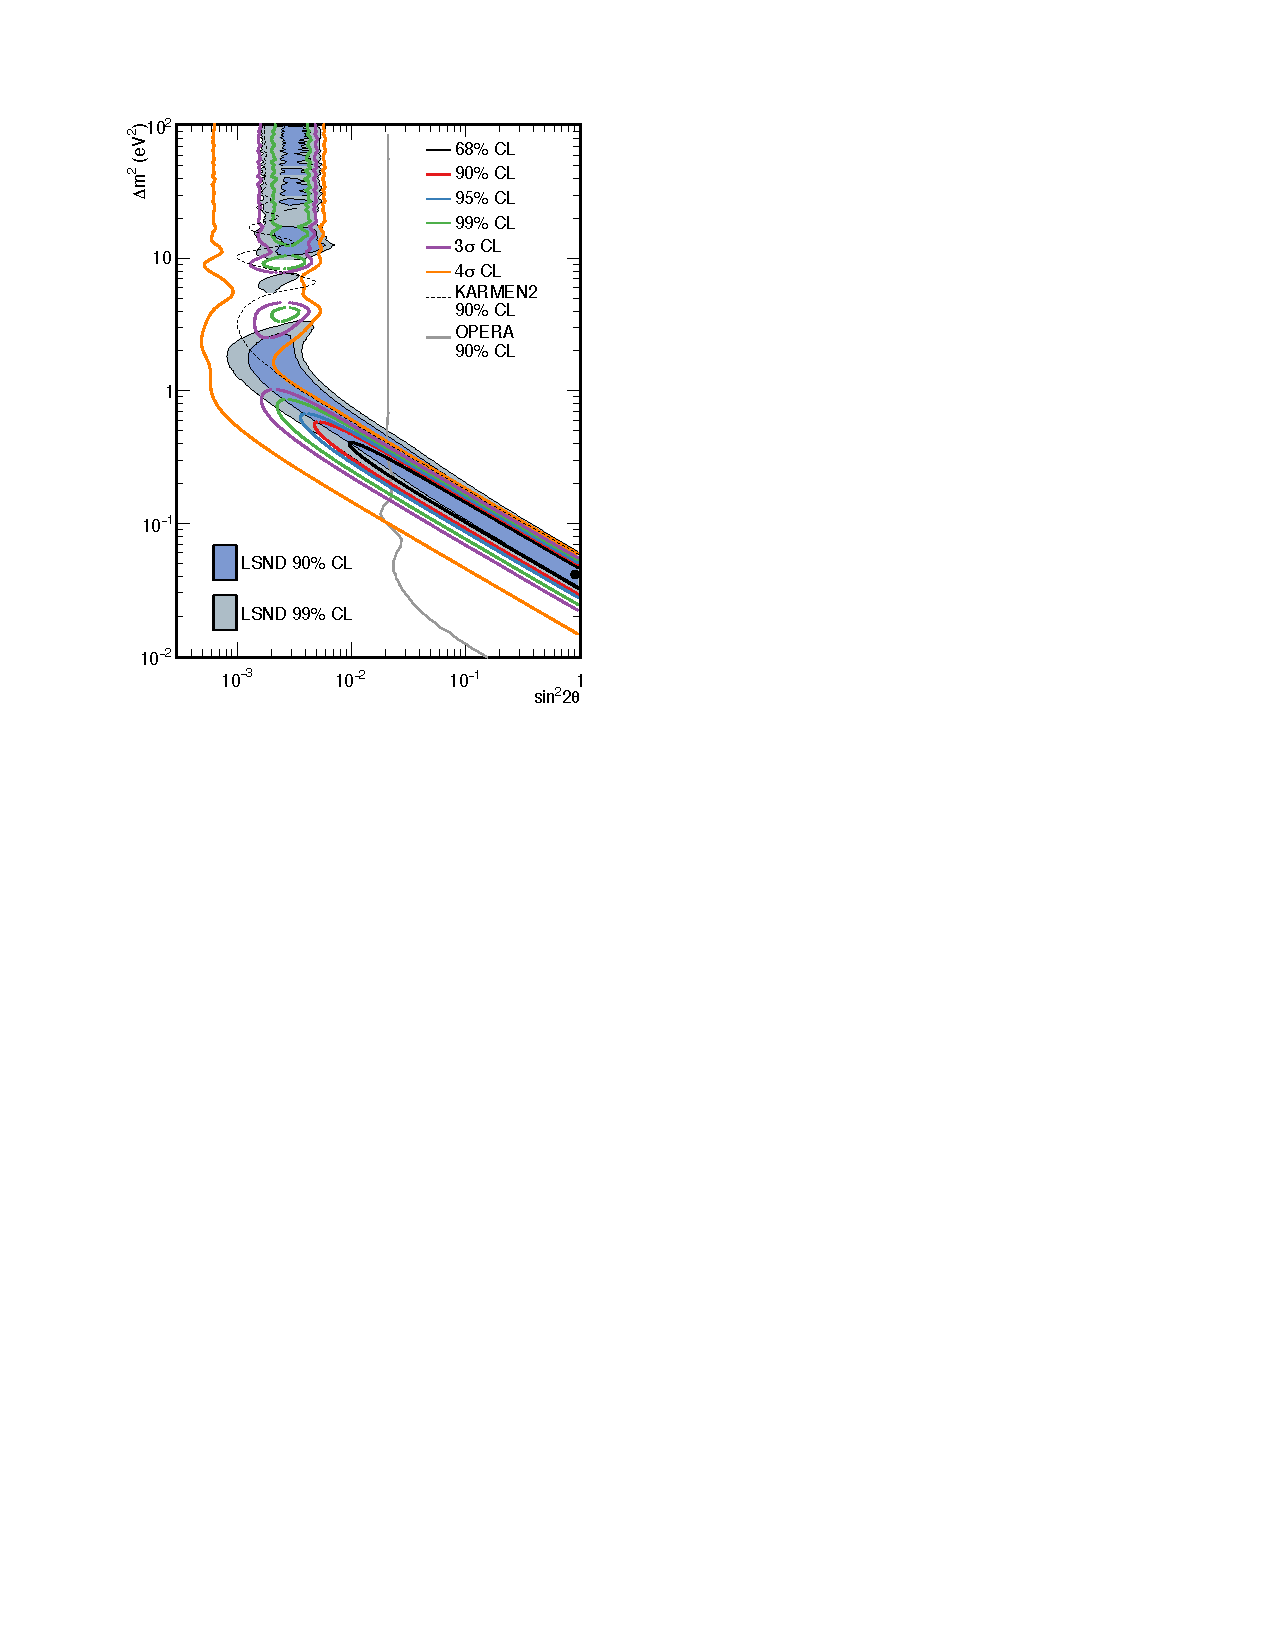
\includegraphics[width=0.7\linewidth]{figures/miniboone_bestfit.pdf}
    \caption{MiniBooNE allowed regions for the combined neutrino mode and antineutrino for events with $200<E_{\nu}^{QE}<3000$~MeV within a two-neutrino oscillation model. The black point at $( \sin^22\theta, \Delta m^2)=(0.96, 0.041~\mathrm{eV^2})$ represents the best fit \cite{Aguilar-Arevalo:2018gpe}.}
    \label{fig:miniboone_bestfit}
\end{figure}

The best fit point, however, is disfavoured by the OPERA $\nu_{e}$ appearance analysis \cite{Agafonova:2018dkb} and by the MINOS, Daya Bay, Bugey-3 combined analysis of $\nu_{\mu}$ disappearance \cite{Adamson:2016jku}. A recent result from IceCube \cite{TheIceCube:2016oqi} further restricts the available parameter space, leaving little room for the $3+1$ hypothesis. As such, other explanations have been proposed for the excess: $3+N$ sterile neutrinos with $N>1$ \cite{Conrad:2012qt}, CPT violation \cite{Kostelecky:2011gq}, and resonant neutrino oscillations \cite{Asaadi:2017bhx} among the others.


\section{Other anomalies}
The LSND and MiniBooNE are not the only two experiments which have observed anomalies in the neutrino sector. Several other experiments obtained results not completely in agreement with the theoretical expectations. In particular, it is possible to identify two categories of anomalies, classified according to the type of the experiment.
\begin{description}
    \item[Radiochemical experiments.] The GALLEX experiment at Gran Sasso and the SAGE experiment at Baksan employed a detection technique similar to the one of Ray Davis experiment at Homestake. In this case, solar neutrino interactions were detected through inverse $\beta$ decay on $^{71}$Ga atoms (instead of $^{37}$Cl):
    \begin{equation}
        \nu_e + ^{71}\mathrm{Ga} \rightarrow e^- + ^{71}\mathrm{Ge}.
    \end{equation}
    The energy threshold for this reaction is 233~keV, which allows to observe the neutrino interactions produced in the solar $pp$ chain reaction (see Figure \ref{fig:solar}). Both experiments observed a deficit of neutrino interactions, which favours with $2.7\sigma$ significance the hypothesis of short-baseline neutrino oscillation \cite{Giunti:2010zu}. Curiously, during the second data-taking run of SAGE, 2 tons of gallium were stolen from the detector (3.6\% of the total mass) \cite{Abdurashitov:1999zd}.
    
    \item[Reactor experiments.]
\end{description} 

Hints for sterile neutrino states have emerged from several neutrino experiments performed with different sources and detectors. None of these measurements offer conclusive evidence for the existence of neutrino oscillations, and measurements which rule out the parameter space of interest to these positive results have also been conducted [17, 18, 19]. All potential signals, if interpreted
1Neutrinos from the early universe are commonly referred to as relic neutrinos. 17
 
as due to oscillations, are compatible with a mass-splitting of order 1 eV 2. We present a short overview of the three main hints for sterile neutrinos, discussing those obtained from accelerator- based measurements in more detail in the following section. A review of experimental results pertaining to sterile neutrino searches, and the analysis methods employed to search for sterile neutrinos is presented in reference [20].

Reactor Anomaly In reactor neutrino experiments a widely observed deficit of a few percent of 1 − 10 MeV e events, uniform in energy, has been hypothesised to be caused by oscillations to a sterile neutrino. Much of the work in understanding the reactor neutrino anomaly involves studying the systematic errors associated to the prediction of the neutrino flux from reactors. The complex chain of fission fragments produced in nuclear reactors, and difficult modeling of atomic transitions makes this an arduous task. A recent measurement by the Daya Bay collaboration [22] seems to attribute, at least in part, the anomaly to the time-dependent composition of the nuclear fuel. A new generation of reactor-neutrino experiments designed to operate at test reactors, where they can be placed much closer to the source, are soon to come online. By taking advantage of the smaller fission core and shorter distance between the core and the detector in such reactor, experiments such as prospect [23] aim to observe the oscillatory L/E dependence of interactions due to a possible sterile neutrino.